\chapter{Трансплантація печінки}

\section{Що таке трансплантація печінки?}

Транспалнтація печінки - це високотехнологічне оперативне втручання, яке полягає у заміні хворої печінки пацієнта на здорову печінку (або частину печінки) донора. 

Після операції пацієнт пожиттєво отримує препарати, які запобігають відторгненню трансплантованого органу.

\begin{tcolorbox}[width=\textwidth,colback=yellow!5!white,colframe=yellow!75!black]    
Реципієнт - людина, якій пересаджують частину печінки
\end{tcolorbox}    

\begin{tcolorbox}[width=\textwidth,colback=yellow!5!white,colframe=yellow!75!black]    
Донор - людина, чию печінку або її частину пересаджують
\end{tcolorbox}    

\section{При яких захворюваннях показана трансплантація печінки?}

Трансплантації печінки показана при кінцевих стадіях захворювань печінки. Найчастіше це цироз печінки в наслідок вірусних гепатитів, аутоімунних захворюваннь печінки, вроджених патологій (біліарна атрезія та ін.), а також деяких нерезектабельних пухлин печінки та при гострій печінковій недостатності.


\section{Які види трансплантації печінки існують?}

За типом донора трансплантація може бути:
\begin{itemize}
    \item трупною, коли у людини з смертю мозку виконують забор цілої печінки
    \item від живого родинного донора, коли частину печінки для трансплантації беруть у живої людини, родича пацієнта 
\end{itemize}

\begin{figure}
  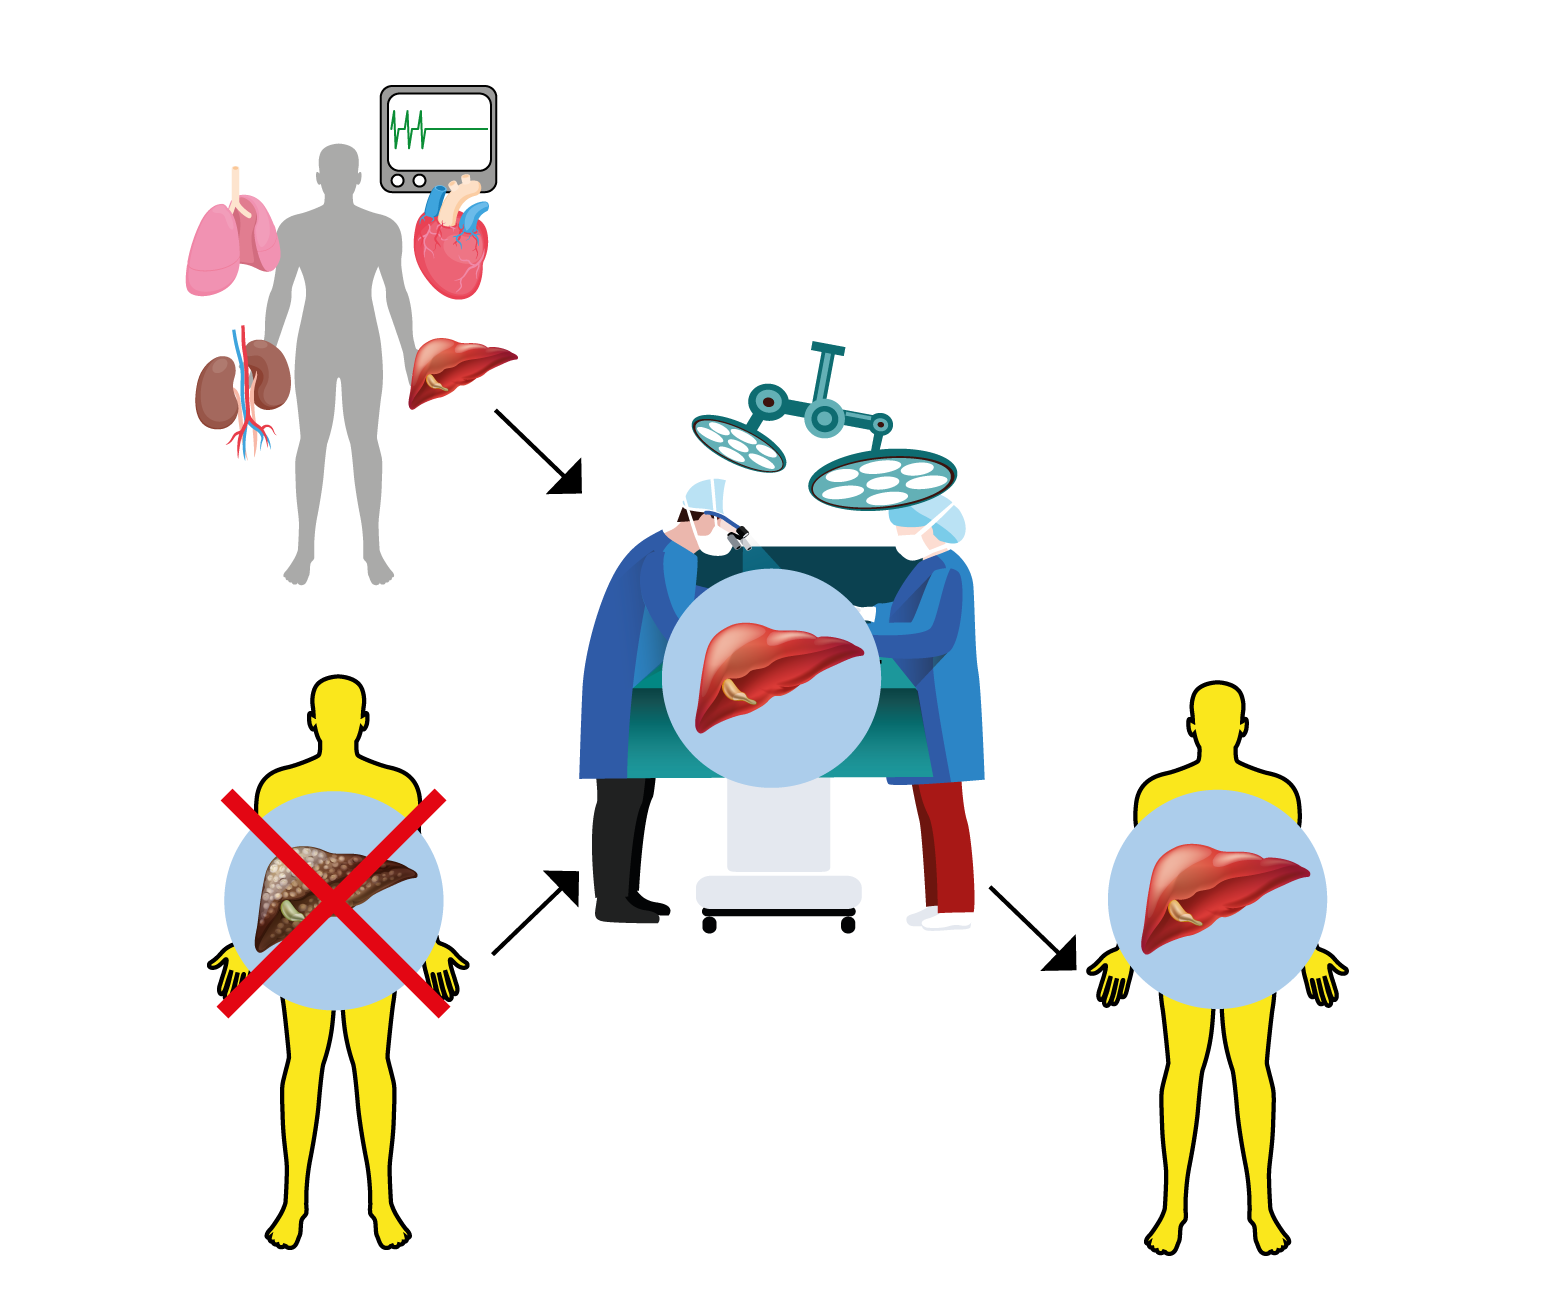
\includegraphics[width=\linewidth]{Figures/LTx-simple_DDLT.png}
%  \checkparity This is an \pageparity\ page.%
  \caption{Трансплантація печінки від трупного донора. В разі отримання згоди від родичів людини із встановленою смертю мозку їй виконують мультиорганний забор, після чого вилучені органи пересаджують ховрому.}
  \label{fig:ddlt}
  %\zsavepos{pos:textfig}
\end{figure}

\begin{figure}
  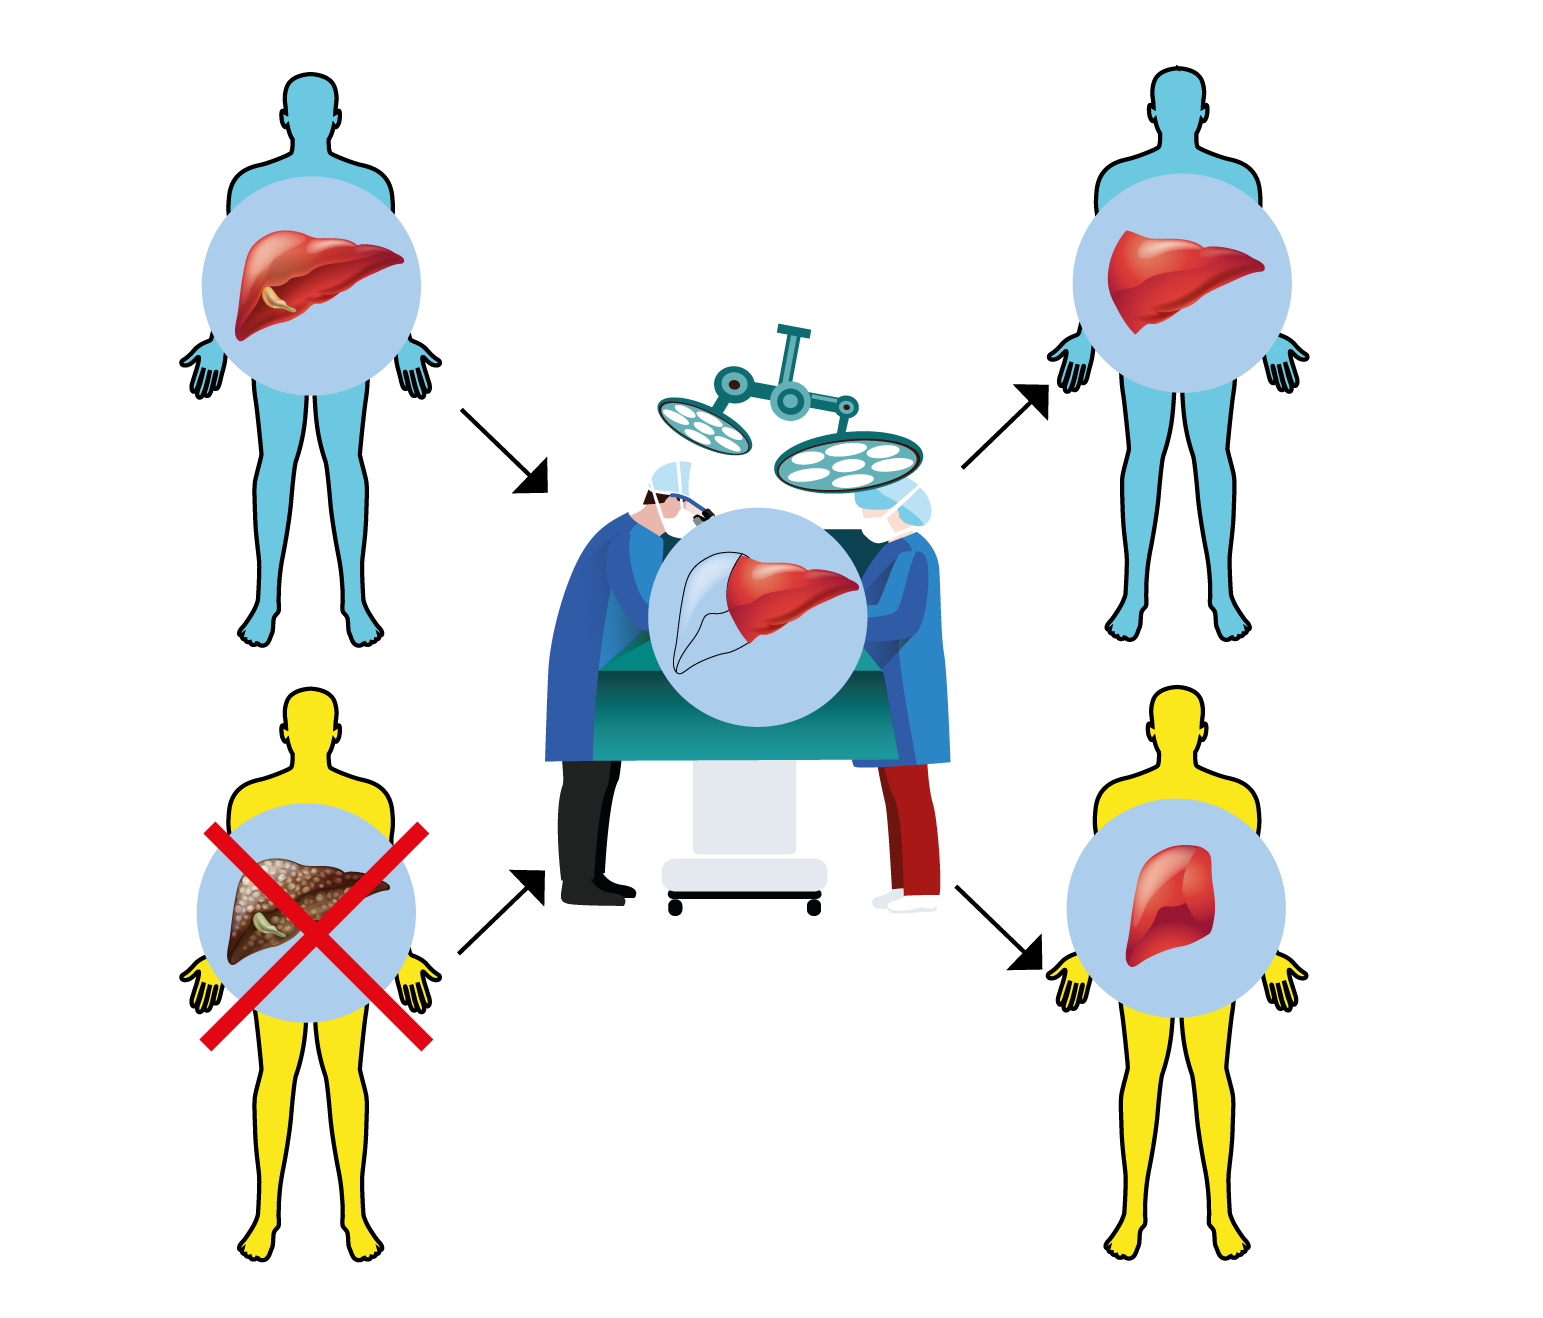
\includegraphics[width=\linewidth]{Figures/LTx-simple_LDLT.png}
%  \checkparity This is an \pageparity\ page.%
  \caption{Трансплантація печінки від живого родинного донора. Родич хворого донує йому частину своєї печінки.}
  \label{fig:ldlt}
  %\zsavepos{pos:textfig}
\end{figure}

Під час забору частини печінки у живого донора його печінку розділяють на дві функціонуючі частини. Одну з них трансплантують реципієнту на те ж місце де знаходилась  печінка, іншу залишають донору.


\section{Хто може бути живим родинним донором печінки?}

Згідно Закону України від 17.05.2018 № 2427-VIII Про застосування трансплантації анатомічних матеріалів людині, донором печінки можуть бути близькі родичі та члени сім’ї, до яких відносяться: чоловік, дружина, батько, мати, вітчим, мачуха, син, дочка, пасинок, падчерка, рідний брат, рідна сестра, двоюрідний брат, двоюрідна сестра, рідна тітка, рідний дядько, рідний племінник, рідна племінниця, дід, баба, прадід, прабаба, внук, внучка, правнук, правнучка, усиновлювач чи усиновлений, опікун чи піклувальник, особа, яка перебуває під опікою або піклуванням, а також особи, які спільно проживають, пов’язані спільним побутом і мають взаємні права та обов’язки, у тому числі особи, які спільно проживають, але не перебувають у шлюбі.



\section{Як відбувається процес підготовки до родинної трансплантації печінки?}

Як трансплантація печінки так і резекція печінки у донора є складними високотехнологічними операціями, тому для їх виконання необхідна ретельна передопераційна підготовка та всебічне поглиблене обстеження обох пацієнтів. В протокол обстеження обов’язково входять комп’ютерна томографія, магнітно-резонансна томографія, колоноскопія, лабораторне дослідження показників крові, та інші дослідження. Після обстеження пацієнти вносяться в лист очікування оперативного втручання